\documentclass[a4paper,11pt]{article}
\usepackage[utf8]{inputenc}
\usepackage[T1]{fontenc}
\usepackage{amsmath,amssymb}
\usepackage[a4paper,left=2cm,right=2cm,top=3.6cm,bottom=2.3cm,headheight=1.1cm,headsep=0.6cm,footskip=1cm]{geometry}
\usepackage{xcolor}
\usepackage{tikz}
\usetikzlibrary{calc,arrows.meta,positioning,shapes.geometric}
\usepackage{fancyhdr}
\usepackage{lastpage}
\usepackage{tabularx}
\usepackage{array}
\usepackage[most]{tcolorbox}
\usepackage{enumitem}
\usepackage{needspace}

% ---------- palet merah dan merah muda ----------
\definecolor{redx}{HTML}{B3202F}
\definecolor{pinkx}{HTML}{E0457B}
\definecolor{maroon}{HTML}{7A1C2C}
\definecolor{softbg}{HTML}{FDF1F4}
\definecolor{salmon}{HTML}{E8836F}
\newcommand{\dis}{\displaystyle}
\renewcommand{\Re}{\operatorname{Re}}
\renewcommand{\Im}{\operatorname{Im}}

\setlength{\parindent}{0pt}
\renewcommand{\arraystretch}{1.35}

\tikzset{
  ar/.style={-{Stealth[length=1.8mm]},thick,redx},
  box/.style={draw=redx,thick,rounded corners=3pt,fill=softbg,align=center,inner sep=4pt}
}

% ---------- header berwarna merah ----------
\pagestyle{fancy}
\fancyhf{}
\renewcommand{\headrulewidth}{0pt}
\fancyhead[L]{%
  \begin{tikzpicture}[remember picture,overlay]
    \fill[redx] ([yshift=-1.2cm]current page.north west) rectangle ([yshift=-3.15cm]current page.north east);
    \fill[pinkx] ([yshift=-3.15cm]current page.north west) rectangle ([yshift=-3.25cm]current page.north east);
  \end{tikzpicture}%
  \color{white}\bfseries\large Latihan Soal Bilangan Kompleks}
\fancyhead[R]{\color{white}\small Diunduh dari website \textbf{Math1729}\ \,|\,\ 4 Oktober 2026}
\fancyfoot[L]{\small\color{redx}Math1729 --- Bilangan Kompleks}
\fancyfoot[R]{\small\color{redx}Halaman \thepage\ dari \pageref{LastPage}}

% ---------- komponen ----------
\newcounter{no}
\newcommand{\bagian}[2]{\par\Needspace{6\baselineskip}\vspace{1.0em}\noindent
  \begin{tcolorbox}[colback=redx,colframe=redx,coltext=white,boxrule=0pt,arc=2pt,left=6pt,right=6pt,top=3pt,bottom=3pt]
  \textbf{#1}\hfill{\small #2}\end{tcolorbox}\setcounter{no}{0}\par\vspace{-0.3em}}
\newcommand{\tingkat}[2]{\par\Needspace{7\baselineskip}\vspace{0.6em}\noindent
  {\color{pinkx}\rule{3pt}{1.1em}}\ {\color{redx}\bfseries #1}\ {\small\color{gray}--- #2}\par\vspace{0.1em}}
\newcommand{\tingkatb}[2]{\par\Needspace{16\baselineskip}\vspace{0.6em}\noindent
  {\color{pinkx}\rule{3pt}{1.1em}}\ {\color{redx}\bfseries #1}\ {\small\color{gray}--- #2}\par\vspace{0.1em}}
\newcommand{\soal}[2]{\par\vspace{0.75em}\stepcounter{no}\noindent
  \begin{minipage}[t]{1.8em}\textbf{\theno.}\end{minipage}%
  \begin{minipage}[t]{\dimexpr\linewidth-1.8em\relax}#1\par\vspace{0.35em}#2\end{minipage}\par}
\newcommand{\poin}[1]{\hfill{\small\color{redx}[#1 poin]}}

% teks di kiri, gambar di kanan
\newcommand{\gbr}[2]{\noindent\begin{minipage}[t]{0.56\linewidth}#1\end{minipage}\hfill\raisebox{\ht\strutbox}{\begin{minipage}[t]{0.41\linewidth}\vspace{0pt}\centering#2\end{minipage}}}

% pilihan jawaban
\newcommand{\pil}[5]{\begin{tabularx}{\linewidth}{@{}*{5}{X}@{}}\textbf{A.}\;#1 & \textbf{B.}\;#2 & \textbf{C.}\;#3 & \textbf{D.}\;#4 & \textbf{E.}\;#5\end{tabularx}}
\newcommand{\pilx}[5]{\begin{tabularx}{\linewidth}{@{}*{3}{X}@{}}\textbf{A.}\;#1 & \textbf{B.}\;#2 & \textbf{C.}\;#3\\[10pt] \textbf{D.}\;#4 & \textbf{E.}\;#5 & \end{tabularx}}
\newcommand{\jwb}{\hfill Jawaban: \rule{4.5cm}{0.4pt}}

\begin{document}
\thispagestyle{fancy}

\begin{center}
  {\color{redx}\fontsize{22}{26}\selectfont\bfseries Latihan Soal Bilangan Kompleks\par}
  \vspace{2pt}
  {\color{pinkx}\large Bentuk $a+bi$, Operasi, Konjugat, Modulus, Argumen, Tafsiran Geometri, dan Persamaan Kuadrat\par}
\end{center}
\vspace{2pt}
\begin{tcolorbox}[colback=softbg,colframe=redx!40,boxrule=0.6pt,arc=3pt,left=8pt,right=8pt,top=5pt,bottom=5pt]
\noindent\textbf{Nama} : \rule{4.6cm}{0.4pt}\hfill\textbf{Kelas} : \rule{2.2cm}{0.4pt}\hfill\textbf{Skor} : \rule{2.2cm}{0.4pt}
\end{tcolorbox}
\vspace{2pt}
\begin{tcolorbox}[colback=white,colframe=pinkx,boxrule=0.8pt,arc=3pt,left=8pt,right=8pt,top=4pt,bottom=4pt,title={\bfseries Petunjuk Pengerjaan},coltitle=white,fonttitle=\small]
\small
\begin{enumerate}[leftmargin=1.4em,itemsep=1pt,topsep=1pt]
\item Soal terdiri atas \textbf{20 pilihan ganda} (5 mudah, 5 sedang, 5 sulit, 5 HOTS), \textbf{5 isian singkat}, dan \textbf{5 uraian (essay)}. Soal disusun berjenjang dari mudah sampai HOTS. Selain pilihan ganda biasa, terdapat bentuk soal yang kini lazim pada UTBK-SNBT dan TKA, yaitu pernyataan benar--salah (kategori), kecukupan data, dan perbandingan kuantitas $P$ dan $Q$. Alokasi waktu yang disarankan: 120 menit.
\item Skor: pilihan ganda 2 poin, isian singkat 4 poin, uraian 8 poin per soal (total 100 poin). Tidak ada pengurangan skor untuk jawaban salah.
\item Notasi: $i^2=-1$; untuk $z=a+bi$ dengan $a,b$ real berlaku $\Re(z)=a$, $\Im(z)=b$, $\bar z=a-bi$, dan $|z|=\sqrt{a^2+b^2}$. Argumen utama $\arg(z)$ berada pada $-\pi<\arg(z)\le\pi$. Pada diagram Argand, sumbu mendatar adalah sumbu real (Re) dan sumbu tegak adalah sumbu imajiner (Im). Gambar tidak selalu digambar sesuai skala.
\item Jawaban isian singkat berupa bilangan atau bilangan kompleks $a+bi$ dalam bentuk paling sederhana.
\item Kalkulator tidak diperkenankan.
\end{enumerate}
\end{tcolorbox}

% =====================================================================
\bagian{A. Pilihan Ganda}{20 soal $\times$ 2 poin = 40 poin. Pilih satu jawaban yang paling tepat.}

\tingkat{Tingkat Mudah}{soal 1 sampai 5}
\soal{Nilai dari $i+i^2+i^3+\cdots+i^{2026}$ adalah \dots.}{\pil{$0$}{$-1$}{$-1+i$}{$1+i$}{$i$}}
\soal{\gbr{Pada diagram Argand di samping, titik $P$ mewakili bilangan kompleks $z$ dan titik $Q$ mewakili bilangan kompleks $w$. Nilai $z+\bar w$ adalah \dots.}{%
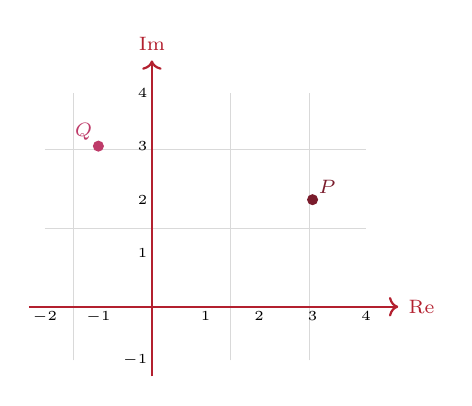
\begin{tikzpicture}[x=0.68cm,y=0.68cm]
\draw[gray!30,very thin] (-2,-1) grid (4,4);
\draw[->,thick,redx] (-2.3,0)--(4.6,0) node[right,font=\scriptsize]{Re};
\draw[->,thick,redx] (0,-1.3)--(0,4.6) node[above,font=\scriptsize]{Im};
\foreach \tk in {-2,-1,1,2,3,4}{\node[font=\tiny,below,inner sep=1.5pt] at (\tk,0) {$\tk$};}
\foreach \tk in {-1,1,2,3,4}{\node[font=\tiny,left,inner sep=1.5pt] at (0,\tk) {$\tk$};}
\fill[maroon] (3,2) circle (2pt) node[above right,font=\scriptsize,inner sep=2pt]{$P$};
\fill[pinkx!85!black] (-1,3) circle (2pt) node[above left,font=\scriptsize,inner sep=2pt]{$Q$};
\end{tikzpicture}}}{\pilx{$2+5i$}{$4-i$}{$2+i$}{$4+5i$}{$2-i$}}
\soal{Bilangan kompleks $z=(x^2-4)+(x+2)i$ dengan $x$ real merupakan bilangan imajiner murni. Nilai $x$ adalah \dots.}{\pilx{$2$}{$-2$}{$0$}{$-2$ atau $2$}{$4$}}
\soal{Jika $z=1-2i$, maka $\dis\frac1z+\frac1{\bar z}=\dots$.}{\pil{$\dis\frac15$}{$\dis\frac{2}{\sqrt5}$}{$\dis\frac45$}{$\dis\frac25$}{$2$}}
\soal{Argumen utama dari bilangan kompleks $z=-\sqrt3+i$ adalah \dots.}{\pil{$\dis\frac\pi6$}{$\dis\frac{5\pi}6$}{$\dis-\frac\pi6$}{$\dis-\frac{5\pi}6$}{$\dis\frac{2\pi}3$}}

\tingkat{Tingkat Sedang}{soal 6 sampai 10}
\soal{Bilangan kompleks $z$ memenuhi $2z-i\bar z=5-i$. Nilai $z^2$ adalah \dots.}{\pil{$10$}{$8-6i$}{$10+6i$}{$6+8i$}{$8+6i$}}
\soal{\gbr{Persamaan $x^2-6x+25=0$ mempunyai akar-akar kompleks $z_1$ dan $z_2$. Pada diagram Argand, titik asal $O$ dan titik-titik yang mewakili $z_1$ dan $z_2$ membentuk sebuah segitiga (daerah arsiran). Luas segitiga tersebut adalah \dots\ satuan luas.}{%
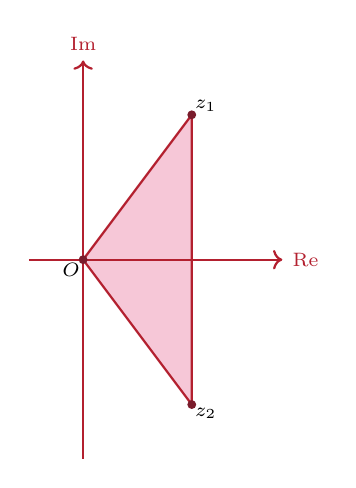
\begin{tikzpicture}[x=0.46cm,y=0.46cm]
\fill[pinkx!30] (0,0)--(3,4)--(3,-4)--cycle;
\draw[->,thick,redx] (-1.5,0)--(5.5,0) node[right,font=\scriptsize]{Re};
\draw[->,thick,redx] (0,-5.5)--(0,5.5) node[above,font=\scriptsize]{Im};
\draw[redx,thick] (0,0)--(3,4)--(3,-4)--cycle;
\fill[maroon] (0,0) circle (1.6pt) (3,4) circle (1.6pt) (3,-4) circle (1.6pt);
\node[font=\scriptsize,below left,inner sep=1pt] at (0,0) {$O$};
\node[font=\scriptsize,above right,inner sep=1pt] at (3,4) {$z_1$};
\node[font=\scriptsize,below right,inner sep=1pt] at (3,-4) {$z_2$};
\end{tikzpicture}}}{\pil{$6$}{$12$}{$18$}{$24$}{$25$}}
\soal{Titik $A$ mewakili bilangan kompleks $z=4+i$. Titik $A$ diputar $90^\circ$ berlawanan arah jarum jam terhadap titik asal, kemudian digeser $2$ satuan ke kiri dan $3$ satuan ke atas sehingga menjadi titik $A'$. Bilangan kompleks yang diwakili $A'$ adalah \dots.}{\pil{$-4+2i$}{$-1-i$}{$1+7i$}{$-3+7i$}{$1+i$}}
\soal{Jika $z=2-i$, maka nilai $z^3-4z^2+7z+2$ adalah \dots.}{\pil{$6-2i$}{$6+2i$}{$2-11i$}{$4-2i$}{$0$}}
\soal{\gbr{Bilangan kompleks $z$ bergerak pada lingkaran berpusat di titik yang mewakili $3+4i$ dan berjari-jari $2$ (lihat gambar). Nilai minimum $|z|$ adalah \dots.}{%
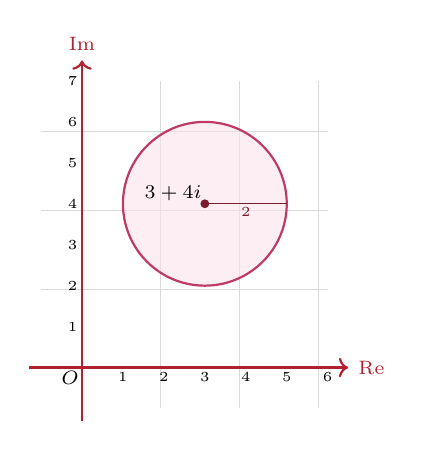
\begin{tikzpicture}[x=0.52cm,y=0.52cm]
\draw[gray!30,very thin] (-1,-1) grid (6,7);
\draw[->,thick,redx] (-1.3,0)--(6.5,0) node[right,font=\scriptsize]{Re};
\draw[->,thick,redx] (0,-1.3)--(0,7.5) node[above,font=\scriptsize]{Im};
\foreach \tk in {1,2,3,4,5,6}{\node[font=\tiny,below,inner sep=1.5pt] at (\tk,0) {$\tk$};}
\foreach \tk in {1,2,3,4,5,6,7}{\node[font=\tiny,left,inner sep=1.5pt] at (0,\tk) {$\tk$};}
\draw[thick,pinkx!85!black,fill=pinkx!15,fill opacity=0.6] (3,4) circle (2);
\fill[maroon] (3,4) circle (1.6pt);
\draw[maroon,thin] (3,4)--(5,4) node[midway,below,font=\tiny,inner sep=1pt]{$2$};
\node[font=\scriptsize,above left,inner sep=1pt] at (3,4) {$3+4i$};
\node[font=\scriptsize,below left,inner sep=1pt] at (0,0) {$O$};
\end{tikzpicture}}}{\pil{$1$}{$2$}{$3$}{$5$}{$7$}}

\tingkat{Tingkat Sulit}{soal 11 sampai 15, setara UTBK}
\soal{Banyaknya bilangan kompleks $z$ yang memenuhi $z^2=\bar z$ adalah \dots.}{\pil{$1$}{$2$}{$3$}{$4$}{$5$}}
\soal{\gbr{Pada diagram Argand, titik $A$ mewakili $1+2i$ dan titik $B$ mewakili $4+3i$. Titik $C$ dan $D$ ditentukan sehingga $ABCD$ adalah persegi dengan urutan titik berlawanan arah jarum jam. Bilangan kompleks yang mewakili titik pusat persegi $ABCD$ adalah \dots.}{%
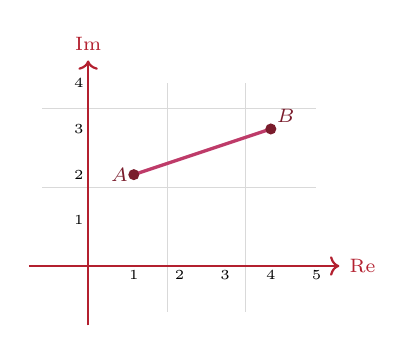
\begin{tikzpicture}[x=0.58cm,y=0.58cm]
\draw[gray!30,very thin] (-1,-1) grid (5,4);
\draw[->,thick,redx] (-1.3,0)--(5.5,0) node[right,font=\scriptsize]{Re};
\draw[->,thick,redx] (0,-1.3)--(0,4.5) node[above,font=\scriptsize]{Im};
\foreach \tk in {1,2,3,4,5}{\node[font=\tiny,below,inner sep=1.5pt] at (\tk,0) {$\tk$};}
\foreach \tk in {1,2,3,4}{\node[font=\tiny,left,inner sep=1.5pt] at (0,\tk) {$\tk$};}
\draw[pinkx!85!black,very thick] (1,2)--(4,3);
\fill[maroon] (1,2) circle (2pt) node[left,font=\scriptsize,inner sep=2pt]{$A$};
\fill[maroon] (4,3) circle (2pt) node[above right,font=\scriptsize,inner sep=2pt]{$B$};
\end{tikzpicture}}}{\pilx{$\dis\frac52+\frac52i$}{$3+3i$}{$2+4i$}{$3+5i$}{$4+4i$}}
\soal{Berapakah nilai $|z|$, jika $z$ adalah bilangan kompleks?
\begin{enumerate}[label=(\arabic*),leftmargin=1.8em,itemsep=0pt,topsep=2pt]
\item $\Re(z)=3$.
\item $z^2=-7+24i$.
\end{enumerate}}{\begin{tabularx}{\linewidth}{@{}lX@{}}
\textbf{A.} & Pernyataan (1) SAJA cukup untuk menjawab pertanyaan, tetapi pernyataan (2) SAJA tidak cukup.\\
\textbf{B.} & Pernyataan (2) SAJA cukup untuk menjawab pertanyaan, tetapi pernyataan (1) SAJA tidak cukup.\\
\textbf{C.} & DUA pernyataan BERSAMA-SAMA cukup untuk menjawab pertanyaan, tetapi SATU pernyataan SAJA tidak cukup.\\
\textbf{D.} & Pernyataan (1) SAJA cukup dan pernyataan (2) SAJA cukup untuk menjawab pertanyaan.\\
\textbf{E.} & Pernyataan (1) dan pernyataan (2) tidak cukup untuk menjawab pertanyaan.
\end{tabularx}}
\soal{Diketahui $z$ bilangan kompleks yang tidak real. Perhatikan dua kuantitas berikut.\par\smallskip
\hspace{1.5em}$P=|z|^2$\hspace{3em}$Q=\Re(z^2)$\par\smallskip
Hubungan antara kuantitas $P$ dan $Q$ adalah \dots.}{\begin{tabularx}{\linewidth}{@{}lX@{}}
\textbf{A.} & $P>Q$\\
\textbf{B.} & $P<Q$\\
\textbf{C.} & $P=Q$\\
\textbf{D.} & Hubungan $P$ dan $Q$ tidak dapat ditentukan.\\
\textbf{E.} & $P$ dan $Q$ tidak dapat dibandingkan karena $Q$ bukan bilangan real.
\end{tabularx}}
\soal{Persamaan suku banyak $z^3-5z^2+17z-13=0$ berkoefisien real dan salah satu akarnya adalah $2+3i$. Jumlah kuadrat semua akarnya adalah \dots.}{\pil{$13$}{$25$}{$-5$}{$9$}{$-9$}}

\tingkat{Tingkat HOTS}{soal 16 sampai 20, penalaran tingkat tinggi gaya UTBK dan TKA}
\soal{Diketahui $z$ bilangan kompleks dengan $|z|=1$. Tentukan setiap pernyataan berikut benar (B) atau salah (S).
\begin{enumerate}[label=(\arabic*),leftmargin=1.8em,itemsep=2pt,topsep=2pt]
\item $\bar z=\dis\frac1z$.
\item $z-\dis\frac1z$ selalu bilangan real.
\item $z+\dis\frac1z$ selalu bilangan real.
\item $|z-1|\ge1$.
\end{enumerate}
Urutan jawaban untuk pernyataan (1), (2), (3), (4) yang tepat adalah \dots.}{\pilx{B, B, B, S}{B, S, S, S}{S, S, B, S}{B, S, B, S}{B, S, B, B}}
\soal{Banyak bilangan asli $n\le100$ sehingga $(1+i)^n$ merupakan bilangan real adalah \dots.}{\pil{$12$}{$25$}{$33$}{$50$}{$100$}}
\soal{Jika $\dis\frac{z-1}{z+1}$ adalah bilangan imajiner murni, maka nilai $|z-1|^2+|z+1|^2$ adalah \dots.}{\pil{$1$}{$2$}{$4$}{$8$}{$16$}}
\soal{Transformasi $T$ pada bidang kompleks didefinisikan oleh $T(z)=iz+3+i$. Titik $z_0=5+2i$ ditransformasikan berulang kali: $z_1=T(z_0)$, $z_2=T(z_1)$, dan seterusnya. Nilai $z_{2026}$ adalah \dots.}{\pil{$5+2i$}{$1+6i$}{$1-2i$}{$1+2i$}{$-3+2i$}}
\soal{Himpunan semua bilangan kompleks $z$ yang memenuhi $|z-1|+|z+1|=2$ pada bidang kompleks berupa \dots.}{\begin{tabularx}{\linewidth}{@{}lX@{}}
\textbf{A.} & ruas garis yang menghubungkan titik $-1$ dan titik $1$\\
\textbf{B.} & lingkaran berpusat di titik asal dengan jari-jari $1$\\
\textbf{C.} & elips dengan fokus di titik $-1$ dan titik $1$\\
\textbf{D.} & seluruh sumbu real\\
\textbf{E.} & himpunan kosong
\end{tabularx}}

% =====================================================================
\bagian{B. Isian Singkat}{5 soal $\times$ 4 poin = 20 poin. Tuliskan hanya jawaban akhir.}

\tingkat{Tingkat Sedang}{soal 1 dan 2}
\soal{Bilangan kompleks $z$ memenuhi $z\bar z=25$ dan $z-\bar z=6i$. Jika $\Re(z)<0$, maka $z=\dots$.}{\jwb}
\soal{Banyak bilangan kompleks $z=a+bi$ dengan $a$ dan $b$ bilangan bulat yang memenuhi $2\le|z|\le3$ adalah \dots.}{\jwb}

\tingkat{Tingkat Sulit}{soal 3 sampai 5}
\soal{Nilai dari $\dis\sum_{k=0}^{2025}k\,i^{k}$ adalah \dots\ (tuliskan dalam bentuk $a+bi$).}{\jwb}
\soal{\gbr{Pada diagram Argand, dua lingkaran masing-masing memiliki persamaan $|z-3|=3$ dan $|z-3i|=3$. Luas daerah irisan kedua lingkaran (daerah arsiran) adalah \dots\ satuan luas (tuliskan dalam bentuk $\pi$).}{%
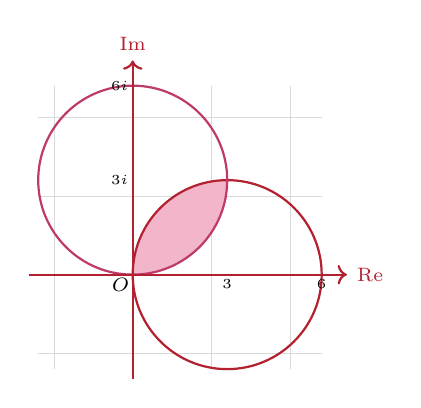
\begin{tikzpicture}[x=0.4cm,y=0.4cm]
\draw[gray!30,very thin] (-3,-3) grid (6,6);
\begin{scope}\clip (3,0) circle (3);\fill[pinkx!40] (0,3) circle (3);\end{scope}
\draw[thick,redx] (3,0) circle (3);
\draw[thick,pinkx!85!black] (0,3) circle (3);
\draw[->,thick,redx] (-3.3,0)--(6.8,0) node[right,font=\scriptsize]{Re};
\draw[->,thick,redx] (0,-3.3)--(0,6.8) node[above,font=\scriptsize]{Im};
\foreach \tk in {3,6}{\node[font=\tiny,below,inner sep=1.5pt] at (\tk,0) {$\tk$};\node[font=\tiny,left,inner sep=1.5pt] at (0,\tk) {$\tk i$};}
\node[font=\scriptsize,below left,inner sep=1pt] at (0,0) {$O$};
\end{tikzpicture}}}{\jwb}
\soal{Jika $\theta$ adalah argumen utama dari $z=(1+i)(\sqrt3+i)$, maka $\tan\theta=\dots$.}{\jwb}

% =====================================================================
\Needspace{16\baselineskip}
\bagian{C. Uraian (Essay)}{5 soal $\times$ 8 poin = 40 poin. Tuliskan langkah penyelesaian dengan lengkap.}

\tingkat{Tingkat Sedang}{soal 1 dan 2}
\soal{\gbr{Sebuah peta bajak laut berbunyi: ``Mulai dari tiang gantungan $G$. Berjalan lurus ke pohon beringin $B$, belok \emph{kanan} $90^\circ$, lalu berjalan sejauh jarak yang sama dan pasang tanda $M_1$. Kembali ke $G$, berjalan lurus ke pohon pinus $P$, belok \emph{kiri} $90^\circ$, berjalan sejauh jarak yang sama dan pasang tanda $M_2$. Harta karun terkubur di tengah-tengah $M_1$ dan $M_2$.'' Pada bidang kompleks (satuan meter), $B=8+2i$ dan $P=2+6i$. Gunakan fakta bahwa mengalikan dengan $i$ memutar $90^\circ$ berlawanan arah jarum jam, dan mengalikan dengan $-i$ memutar $90^\circ$ searah jarum jam.\par\smallskip
(a) Jika $G$ berada di titik asal, tentukan bilangan kompleks yang mewakili $M_1$ dan $M_2$.\par
(b) Tentukan letak harta karun.\par
(c) Tiang gantungan ternyata telah pindah ke $G'=-3+5i$. Tentukan letak harta karun dengan prosedur yang sama, lalu bandingkan dengan hasil (b).\par
(d) Misalkan tiang gantungan berada di titik sembarang $g$. Buktikan bahwa letak harta karun tidak bergantung pada $g$, lalu nyatakan letaknya dalam $b$ dan $p$.}{%
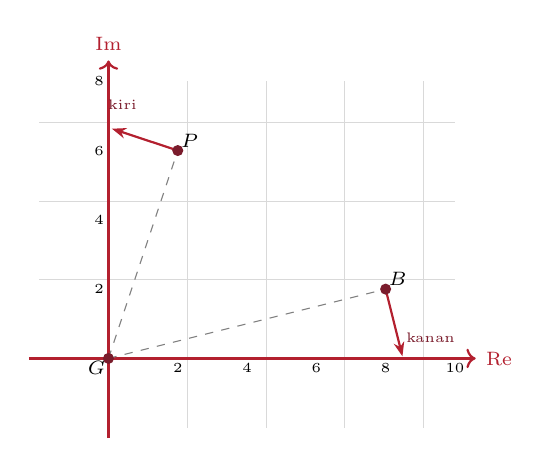
\begin{tikzpicture}[x=0.44cm,y=0.44cm]
\draw[gray!30,very thin] (-2,-2) grid (10,8);
\draw[->,thick,redx] (-2.3,0)--(10.6,0) node[right,font=\scriptsize]{Re};
\draw[->,thick,redx] (0,-2.3)--(0,8.6) node[above,font=\scriptsize]{Im};
\foreach \tk in {2,4,6,8,10}{\node[font=\tiny,below,inner sep=1.5pt] at (\tk,0) {$\tk$};}
\foreach \tk in {2,4,6,8}{\node[font=\tiny,left,inner sep=1.5pt] at (0,\tk) {$\tk$};}
\draw[gray,dashed] (0,0)--(8,2);
\draw[gray,dashed] (0,0)--(2,6);
\draw[ar] (8,2)--++(0.485,-1.94);
\draw[ar] (2,6)--++(-1.9,0.63);
\fill[maroon] (0,0) circle (2pt) (8,2) circle (2pt) (2,6) circle (2pt);
\node[font=\scriptsize,below left,inner sep=1pt] at (0,0) {$G$};
\node[font=\scriptsize,above right,inner sep=1pt] at (8,2) {$B$};
\node[font=\scriptsize,above right,inner sep=1pt] at (2,6) {$P$};
\node[font=\tiny,maroon,right,inner sep=1pt] at (8.5,0.6) {kanan};
\node[font=\tiny,maroon,above,inner sep=1pt] at (0.4,7.1) {kiri};
\end{tikzpicture}}}{\poin{8}}
\soal{Perhatikan persamaan kuadrat berkoefisien kompleks $z^2-3z+(3+i)=0$.\par\smallskip
(a) Tentukan semua bilangan kompleks $w$ yang memenuhi $w^2=-3-4i$.\par
(b) Hitung diskriminan $D=b^2-4ac$ persamaan tersebut, lalu gunakan hasil (a) untuk menentukan kedua akarnya, $z_1$ dan $z_2$.\par
(c) Periksa jawaban Anda dengan rumus jumlah dan hasil kali akar-akar.\par
(d) Pada persamaan kuadrat berkoefisien real, akar-akar yang tidak real selalu saling konjugat. Apakah $z_2=\bar z_1$ di sini? Jelaskan alasannya, lalu tentukan persamaan kuadrat yang akar-akarnya $\bar z_1$ dan $\bar z_2$.}{\poin{8}}

\tingkatb{Tingkat Sulit}{soal 3 dan 4}
\soal{\gbr{Dua menara pemancar berada di titik asal $O$ dan di titik $A$ yang mewakili $3i$ pada bidang kompleks (satuan km). Sinyal menara $O$ dianggap lebih kuat daripada menara $A$ di titik $z$ jika jarak $z$ ke $A$ paling sedikit dua kali jarak $z$ ke $O$, yaitu $|z-3i|\ge2|z|$.\par\smallskip
(a) Tunjukkan bahwa titik-titik $z$ dengan $|z-3i|=2|z|$ membentuk sebuah lingkaran, lalu tentukan pusat dan jari-jarinya.\par
(b) Ujilah titik $O$ untuk menentukan daerah yang memenuhi $|z-3i|\ge2|z|$, lalu hitung luas daerah tersebut.\par
(c) Tentukan jarak terdekat dan terjauh dari $O$ ke batas daerah, beserta bilangan kompleks pada batas yang bersesuaian.\par
(d) Tentukan semua bilangan kompleks $z$ pada batas daerah yang bagian realnya $\sqrt3$.}{%
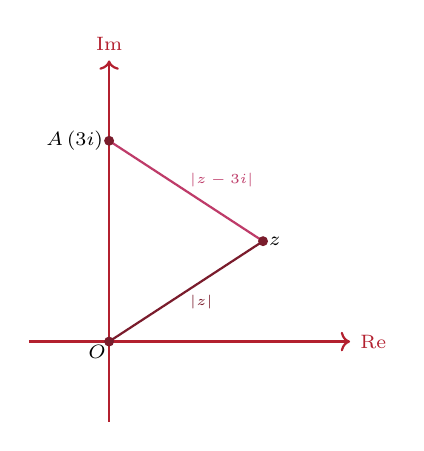
\begin{tikzpicture}[x=0.85cm,y=0.85cm]
\draw[->,thick,redx] (-1.2,0)--(3.6,0) node[right,font=\scriptsize]{Re};
\draw[->,thick,redx] (0,-1.2)--(0,4.2) node[above,font=\scriptsize]{Im};
\coordinate (O) at (0,0); \coordinate (A) at (0,3); \coordinate (Z) at (2.3,1.5);
\draw[maroon,thick] (O)--(Z) node[midway,below right,font=\tiny,inner sep=1pt]{$|z|$};
\draw[pinkx!85!black,thick] (A)--(Z) node[midway,above right,font=\tiny,inner sep=1pt]{$|z-3i|$};
\fill[maroon] (O) circle (1.8pt) (A) circle (1.8pt) (Z) circle (1.8pt);
\node[font=\scriptsize,below left,inner sep=1pt] at (O) {$O$};
\node[font=\scriptsize,left,inner sep=2pt] at (A) {$A\,(3i)$};
\node[font=\scriptsize,right,inner sep=2pt] at (Z) {$z$};
\end{tikzpicture}}}{\poin{8}}
\soal{Diketahui bilangan kompleks $z\neq0$.\par\smallskip
(a) Buktikan bahwa $z+\dis\frac1z$ bilangan real jika dan hanya jika $z$ real atau $|z|=1$. (Petunjuk: tulis $z=x+yi$ dan hitung bagian imajiner $z+\frac1z$.)\par
(b) Selesaikan $z+\dis\frac1z=\frac52$.\par
(c) Selesaikan $z+\dis\frac1z=\frac32$, lalu hitung $|z|$ untuk setiap akar.\par
(d) Misalkan $k$ real. Dengan memakai (a), tunjukkan bahwa jika $|k|<2$ maka setiap akar persamaan $z+\frac1z=k$ memenuhi $|z|=1$, sedangkan jika $|k|\ge2$ maka semua akarnya real.}{\poin{8}}

\Needspace{28\baselineskip}
\tingkatb{Tingkat HOTS}{soal 5}
\soal{\gbr{Dalam grafika komputer, bilangan kompleks $c$ diuji dengan barisan $z_0=0$ dan $z_{n+1}=z_n^2+c$. Titik $c$ disebut \emph{terikat} jika barisan tersebut tidak tumbuh tanpa batas. Dua fakta yang boleh dipakai: (i) jika suatu suku memenuhi $|z_n|>2$, barisan pasti tidak terikat; (ii) jika barisan mulai berulang secara periodik, $c$ terikat. Gambar memperlihatkan lingkaran $|z|=2$ dan empat bilangan $c$ yang akan diuji.\par\smallskip
(a) Untuk $c=-1$, hitung $z_1,z_2,z_3,z_4$. Apakah $c$ terikat?\par
(b) Untuk $c=i$, hitung $z_1,z_2,\dots,z_5$. Apakah $c$ terikat? Jelaskan.\par
(c) Untuk $c=1$ dan $c=1+i$, tentukan $n$ terkecil sehingga $|z_n|>2$.\par
(d) Misalkan $c$ real dan $c>\frac14$. Buktikan $z_n\ge n\left(c-\frac14\right)$ untuk semua $n\ge0$, sehingga $c$ tidak terikat. (Petunjuk: lengkapkan kuadrat untuk menunjukkan $z_{n+1}-z_n\ge c-\frac14$.)}{%
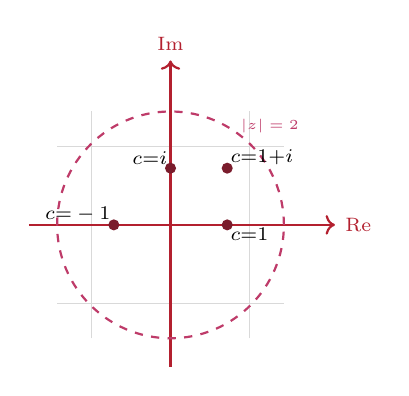
\begin{tikzpicture}[x=0.72cm,y=0.72cm]
\draw[gray!30,very thin] (-2,-2) grid (2,2);
\draw[->,thick,redx] (-2.5,0)--(2.9,0) node[right,font=\scriptsize]{Re};
\draw[->,thick,redx] (0,-2.5)--(0,2.9) node[above,font=\scriptsize]{Im};
\draw[dashed,pinkx!85!black,thick] (0,0) circle (2);
\node[font=\tiny,pinkx!85!black] at (1.75,1.75) {$|z|=2$};
\fill[maroon] (-1,0) circle (2pt) (0,1) circle (2pt) (1,0) circle (2pt) (1,1) circle (2pt);
\node[font=\scriptsize,above left,inner sep=1pt] at (-1,0) {$c{=}-1$};
\node[font=\scriptsize,above left,inner sep=1pt] at (0,1) {$c{=}i$};
\node[font=\scriptsize,below right,inner sep=1pt] at (1,0) {$c{=}1$};
\node[font=\scriptsize,above right,inner sep=1pt] at (1,1) {$c{=}1{+}i$};
\end{tikzpicture}}}{\poin{8}}

% =====================================================================
\newpage
\bagian{Kunci Jawaban dan Pembahasan Singkat}{Untuk guru dan pembahasan mandiri}
\par\vspace{0.6em}{\bfseries\color{redx}Kunci Pilihan Ganda}\par\vspace{0.3em}
\small
\begin{tabularx}{\linewidth}{@{}*{10}{>{\centering\arraybackslash}X}@{}}\hline \textbf{1} & \textbf{2} & \textbf{3} & \textbf{4} & \textbf{5} & \textbf{6} & \textbf{7} & \textbf{8} & \textbf{9} & \textbf{10}\\ \hline C & E & A & D & B & E & B & D & A & C\\ \hline\end{tabularx}\\[6pt]
\begin{tabularx}{\linewidth}{@{}*{10}{>{\centering\arraybackslash}X}@{}}\hline \textbf{11} & \textbf{12} & \textbf{13} & \textbf{14} & \textbf{15} & \textbf{16} & \textbf{17} & \textbf{18} & \textbf{19} & \textbf{20}\\ \hline D & C & B & A & E & D & B & C & E & A\\ \hline\end{tabularx}
\par\vspace{0.8em}{\bfseries\color{redx}\normalsize Pembahasan Pilihan Ganda}\par\vspace{0.2em}
\small\begin{enumerate}[leftmargin=2em,itemsep=2pt,topsep=2pt]
\item[\textbf{1.}] \textbf{(C)} Empat suku berurutan berjumlah nol: $i+i^2+i^3+i^4=i-1-i+1=0$. Dari $i^1$ sampai $i^{2024}$ ada $506$ kelompok yang masing-masing bernilai $0$. Sisanya $i^{2025}+i^{2026}=i+(-1)=-1+i$. (Jebakan: $0$ jika mengira semua suku habis dikelompokkan; $-1$ jika lupa $i^{2025}$.)
\item[\textbf{2.}] \textbf{(E)} Dari diagram, $z=3+2i$ dan $w=-1+3i$, sehingga $\bar w=-1-3i$. Maka $z+\bar w=(3-1)+(2-3)i=2-i$. (Jebakan: A adalah $z+w$, B adalah $z-w$, C adalah $\bar z+w$.)
\item[\textbf{3.}] \textbf{(A)} Imajiner murni berarti bagian real $=0$ dan bagian imajiner $\neq0$. Dari $x^2-4=0$ diperoleh $x=\pm2$. Untuk $x=-2$ bagian imajiner $x+2=0$, sehingga $z=0$ yang bukan imajiner murni. Jadi $x=2$ dan $z=4i$.
\item[\textbf{4.}] \textbf{(D)} $\dis\frac1z+\frac1{\bar z}=\frac{z+\bar z}{z\bar z}=\frac{2\Re(z)}{|z|^2}=\frac{2\cdot1}{5}=\frac25$. Cek langsung: $\frac1z=\frac{1+2i}{5}$ dan $\frac1{\bar z}=\frac{1-2i}{5}$.
\item[\textbf{5.}] \textbf{(B)} Titik $(-\sqrt3,1)$ berada di kuadran II dengan sudut acuan $\alpha=\arctan\dis\frac{1}{\sqrt3}=\frac\pi6$. Maka $\arg(z)=\pi-\frac\pi6=\frac{5\pi}6$. (Jebakan: A mengabaikan kuadran; C dan D salah kuadran.)
\item[\textbf{6.}] \textbf{(E)} Misalkan $z=x+yi$. Maka $2z-i\bar z=2x+2yi-i(x-yi)=(2x-y)+(2y-x)i$. Dari $2x-y=5$ dan $2y-x=-1$ diperoleh $y=1$ dan $x=3$, jadi $z=3+i$ dan $z^2=9+6i-1=8+6i$.
\item[\textbf{7.}] \textbf{(B)} Akar-akarnya $x=\dis\frac{6\pm\sqrt{36-100}}{2}=3\pm4i$. Titik-titiknya $O(0,0)$, $(3,4)$, dan $(3,-4)$. Alas segitiga adalah ruas yang menghubungkan $(3,4)$ dan $(3,-4)$ sepanjang $8$, dan tinggi $=3$ (jarak $O$ ke garis $\Re(z)=3$). Luas $=\frac12\cdot8\cdot3=12$. (Jebakan D: lupa faktor $\frac12$.)
\item[\textbf{8.}] \textbf{(D)} Putar: $i(4+i)=-1+4i$. Geser $-2+3i$: $(-1+4i)+(-2+3i)=-3+7i$. Jebakan: A (geser dahulu baru putar) $i\big((4+i)+(-2+3i)\big)=-4+2i$; B (putar searah jarum jam) $-i(4+i)+(-2+3i)=-1-i$; C (salah arah geser horizontal) $1+7i$; E (salah arah geser vertikal) $1+i$.
\item[\textbf{9.}] \textbf{(A)} Karena $z=2-i$ adalah akar $x^2-4x+5=0$, berlaku $z^2-4z+5=0$. Maka $z^3-4z^2+7z+2=z(z^2-4z+5)+2z+2=2z+2=6-2i$. Cek langsung: $z^2=3-4i$ dan $z^3=2-11i$, sehingga $(2-11i)-4(3-4i)+7(2-i)+2=6-2i$.
\item[\textbf{10.}] \textbf{(C)} Jarak pusat $3+4i$ ke titik asal adalah $5$. Dengan ketaksamaan segitiga, $|z|\ge|3+4i|-|z-(3+4i)|=5-2=3$, dan kesamaan tercapai di titik lingkaran yang terletak pada ruas $O$ ke pusat. Nilai maksimumnya $5+2=7$.
\item[\textbf{11.}] \textbf{(D)} Misalkan $z=x+yi$. Dari $z^2=\bar z$: $x^2-y^2=x$ dan $2xy=-y$. Persamaan kedua memberi $y=0$ atau $x=-\frac12$. Jika $y=0$: $x^2=x$, sehingga $z=0$ atau $z=1$. Jika $x=-\frac12$: $\frac14-y^2=-\frac12$, sehingga $y=\pm\frac{\sqrt3}{2}$, yaitu dua bilangan. Total $4$. (Jebakan: lupa $z=0$ atau lupa kasus $y=0$.)
\item[\textbf{12.}] \textbf{(C)} $\overrightarrow{AB}=b-a=3+i$. Memutar $\overrightarrow{AB}$ sebesar $90^\circ$ berlawanan arah jarum jam memberi $\overrightarrow{AD}=i(3+i)=-1+3i$, sehingga $d=a+\overrightarrow{AD}=5i$ dan $c=b+\overrightarrow{AD}=3+6i$. Pusat persegi adalah titik tengah diagonal $AC$: $\frac{(1+2i)+(3+6i)}{2}=2+4i$. Cek dengan diagonal $BD$: $\frac{(4+3i)+5i}{2}=2+4i$. (Jebakan A: titik tengah sisi $AB$.)
\item[\textbf{13.}] \textbf{(B)} Pernyataan (1) saja: hanya diketahui bagian real, sedangkan bagian imajiner bebas, sehingga $|z|$ tidak tertentu. Pernyataan (2) saja: $|z|^2=|z^2|=|-7+24i|=25$, sehingga $|z|=5$ (cukup, tanpa perlu mencari $z$). Jadi hanya (2) yang cukup.
\item[\textbf{14.}] \textbf{(A)} Misalkan $z=x+yi$ dengan $y\neq0$. Maka $P=x^2+y^2$ dan $Q=\Re(z^2)=x^2-y^2$, sehingga $P-Q=2y^2>0$ dan $P>Q$. (Jebakan C dan D: kasus $z$ real memberi $P=Q$, tetapi soal menyatakan $z$ tidak real. Jebakan E: $Q$ adalah bagian real, jadi tetap bilangan real.)
\item[\textbf{15.}] \textbf{(E)} Koefisien real, sehingga konjugat $2-3i$ juga akar. Jumlah ketiga akar adalah $5$, sehingga akar ketiga $=5-4=1$. Jumlah kuadrat: $1^2+(2+3i)^2+(2-3i)^2=1+(-5+12i)+(-5-12i)=-9$. Cek dengan Vieta: $(\sum z)^2-2\sum z_jz_k=25-2\cdot17=-9$.
\item[\textbf{16.}] \textbf{(D)} (1) \emph{Benar}: $z\bar z=|z|^2=1$, sehingga $\bar z=\frac1z$. (2) \emph{Salah}: $z-\frac1z=z-\bar z=2\Im(z)\,i$ adalah imajiner murni; contoh $z=i$ memberi $i-\frac1i=2i$. (3) \emph{Benar}: $z+\frac1z=z+\bar z=2\Re(z)$ bilangan real. (4) \emph{Salah}: untuk $z=\frac{\sqrt3}{2}+\frac12i$, $|z-1|=\sqrt{\left(1-\frac{\sqrt3}2\right)^2+\frac14}=\sqrt{2-\sqrt3}\approx0{,}52<1$. Urutan: B, S, B, S.
\item[\textbf{17.}] \textbf{(B)} $(1+i)^2=2i$. Untuk $n=2k$: $(1+i)^n=2^ki^k$, real jika dan hanya jika $k$ genap, yaitu $n$ kelipatan $4$. Untuk $n$ ganjil: $(1+i)^n=2^ki^k(1+i)$ dan $i^k(1+i)\in\{1+i,\,-1+i,\,-1-i,\,1-i\}$, tidak pernah real. Kelipatan $4$ dari $1$ sampai $100$ ada $25$. (Jebakan D: menghitung semua $n$ genap.)
\item[\textbf{18.}] \textbf{(C)} $\dis\frac{z-1}{z+1}=\frac{(z-1)(\bar z+1)}{|z+1|^2}=\frac{(|z|^2-1)+2\Im(z)\,i}{|z+1|^2}$. Imajiner murni berarti $|z|^2-1=0$, jadi $|z|=1$. Maka $|z-1|^2+|z+1|^2=(z-1)(\bar z-1)+(z+1)(\bar z+1)=2|z|^2+2=4$. (Tafsiran geometri: $z$ pada lingkaran berdiameter dari $-1$ sampai $1$, sehingga segitiga siku-siku di $z$ dan $|z-1|^2+|z+1|^2=2^2$.)
\item[\textbf{19.}] \textbf{(E)} Titik tetap $c$ memenuhi $c=ic+3+i$, sehingga $c=\frac{3+i}{1-i}=\frac{(3+i)(1+i)}{2}=1+2i$. Karena $T(z)-c=i(z-c)$, $T$ adalah rotasi $90^\circ$ berlawanan arah jarum jam terhadap $c=1+2i$. Maka $z_n=c+i^n(z_0-c)=1+2i+4i^n$. Karena $2026=4\cdot506+2$, $i^{2026}=-1$ dan $z_{2026}=1+2i-4=-3+2i$. (Pilihan lain adalah $z_0$, $z_1$, $z_3$, dan pusat rotasi.)
\item[\textbf{20.}] \textbf{(A)} $|z-1|$ dan $|z+1|$ adalah jarak $z$ ke titik $1$ dan $-1$, yang terpisah sejauh $2$. Menurut ketaksamaan segitiga, $|z-1|+|z+1|\ge|(z+1)-(z-1)|=2$, dengan kesamaan jika dan hanya jika $z$ terletak pada ruas yang menghubungkan $-1$ dan $1$. Elips baru terbentuk jika jumlah jarak lebih dari $2$.
\end{enumerate}
\par\Needspace{6\baselineskip}\vspace{0.6em}{\bfseries\color{redx}\normalsize Pembahasan Isian Singkat}\par\vspace{0.2em}
\small\begin{enumerate}[leftmargin=2em,itemsep=2pt,topsep=2pt]
\item[\textbf{1.}] \textbf{Jawaban: $-4+3i$.} Misalkan $z=x+yi$. Dari $z-\bar z=2yi=6i$ diperoleh $y=3$. Dari $z\bar z=x^2+9=25$ diperoleh $x=\pm4$. Karena $\Re(z)<0$, $x=-4$.
\item[\textbf{2.}] \textbf{Jawaban: $20$.} Syarat: $4\le a^2+b^2\le9$. Nilai $a^2+b^2=4$: $(\pm2,0),(0,\pm2)$ ada $4$. Nilai $5$: $(\pm1,\pm2),(\pm2,\pm1)$ ada $8$. Nilai $8$: $(\pm2,\pm2)$ ada $4$. Nilai $9$: $(\pm3,0),(0,\pm3)$ ada $4$. Nilai $6$ dan $7$ tidak mungkin. Total $4+8+4+4=20$.
\item[\textbf{3.}] \textbf{Jawaban: $1012+1013i$.} Untuk setiap empat suku: $4m\cdot1+(4m+1)i-(4m+2)-(4m+3)i=-2-2i$. Suku $k=0$ sampai $2023$ membentuk $506$ kelompok, jumlahnya $506(-2-2i)=-1012-1012i$. Sisanya $k=2024$: $2024\,i^{2024}=2024$ dan $k=2025$: $2025\,i$. Jumlah $=(2024-1012)+(2025-1012)i=1012+1013i$.
\item[\textbf{4.}] \textbf{Jawaban: $\dis\frac{9\pi}{2}-9$.} Pusat lingkaran $3$ dan $3i$, masing-masing berjari-jari $3$, dan keduanya berpotongan di $0$ dan $3+3i$. Tali busur persekutuan $=3\sqrt2$ dan $2\cdot3\sin\frac\theta2=3\sqrt2$ memberi $\theta=90^\circ$. Satu tembereng $=\frac14\pi\cdot3^2-\frac12\cdot3\cdot3=\frac{9\pi}4-\frac92$. Irisan terdiri atas dua tembereng kongruen: $2\left(\frac{9\pi}4-\frac92\right)=\frac{9\pi}2-9$.
\item[\textbf{5.}] \textbf{Jawaban: $2+\sqrt3$.} $z=(1+i)(\sqrt3+i)=(\sqrt3-1)+(\sqrt3+1)i$, di kuadran I. $\tan\theta=\dis\frac{\sqrt3+1}{\sqrt3-1}=\frac{(\sqrt3+1)^2}{2}=\frac{4+2\sqrt3}{2}=2+\sqrt3$ (yaitu $\theta=75^\circ$).
\end{enumerate}
\par\Needspace{8\baselineskip}\vspace{0.6em}{\bfseries\color{redx}\normalsize Pembahasan dan Pedoman Penskoran Uraian}\par\vspace{0.2em}
\small\begin{enumerate}[leftmargin=2em,itemsep=3pt,topsep=2pt]
\item[\textbf{1.}] (a) Dengan $g=0$: $M_1=B+(-i)(B-0)=(1-i)B=(1-i)(8+2i)=10-6i$ dan $M_2=P+i(P-0)=(1+i)P=(1+i)(2+6i)=-4+8i$. (b) Harta karun di titik tengah: $\frac{(10-6i)+(-4+8i)}{2}=3+i$, yaitu $3$ m ke kanan dan $1$ m ke atas dari titik asal. (c) $M_1=B-i(B-G')=8+2i-i(11-3i)=5-9i$ dan $M_2=P+i(P-G')=2+6i+i(5+i)=1+11i$. Titik tengahnya $\frac{6+2i}{2}=3+i$, sama dengan (b). (d) $M_1=b-i(b-g)$ dan $M_2=p+i(p-g)$. Jumlahnya $M_1+M_2=b+p+i(p-b)+(ig-ig)=b+p+i(p-b)$, suku $g$ saling meniadakan. Jadi harta karun di $T=\dfrac{b+p+i(p-b)}{2}=\dfrac{(1-i)b+(1+i)p}{2}$ yang tidak memuat $g$. Cek: $\frac{(1-i)(8+2i)+(1+i)(2+6i)}{2}=3+i$. \\ \textit{Penskoran: (a) 2 poin; (b) 2 poin; (c) 2 poin; (d) 2 poin.}
\item[\textbf{2.}] (a) Misalkan $w=x+yi$. Dari $w^2=-3-4i$: $x^2-y^2=-3$ dan $2xy=-4$. Substitusi $y=-\frac2x$: $x^4+3x^2-4=0\Rightarrow(x^2+4)(x^2-1)=0\Rightarrow x=\pm1$. Jadi $w=1-2i$ atau $w=-1+2i$, yaitu $w=\pm(1-2i)$. (b) $D=(-3)^2-4(3+i)=-3-4i$, sehingga $\sqrt D=\pm(1-2i)$. Akar-akarnya $z=\frac{3\pm(1-2i)}{2}$, yaitu $z_1=2-i$ dan $z_2=1+i$. (c) $z_1+z_2=3$ dan $z_1z_2=(2-i)(1+i)=2+2i-i-i^2=3+i$, sesuai dengan $-\frac ba=3$ dan $\frac ca=3+i$. (d) $\bar z_1=2+i\neq z_2=1+i$, jadi $z_2\neq\bar z_1$. Sifat akar-akar konjugat hanya berlaku bila koefisien real; di sini koefisien $3+i$ tidak real. Akar-akar $\bar z_1=2+i$ dan $\bar z_2=1-i$ memiliki jumlah $3$ dan hasil kali $(2+i)(1-i)=3-i$, sehingga persamaannya $z^2-3z+(3-i)=0$ (koefisiennya dikonjugatkan). \\ \textit{Penskoran: (a) 2 poin; (b) 2 poin; (c) 2 poin; (d) 2 poin.}
\item[\textbf{3.}] (a) Misalkan $z=x+yi$. $|z-3i|^2=4|z|^2\Rightarrow x^2+(y-3)^2=4x^2+4y^2\Rightarrow3x^2+3y^2+6y-9=0\Rightarrow x^2+(y+1)^2=4$. Lingkaran berpusat di $-i$ dengan jari-jari $2$. (b) Uji $O$: $|0-3i|=3\ge2\cdot0$ benar, jadi $O$ termasuk daerah. $O$ berada di dalam lingkaran (jarak ke pusat $1<2$), sehingga daerahnya adalah cakram beserta batasnya dengan luas $\pi\cdot2^2=4\pi$ km$^2$. (c) Jarak $O$ ke pusat $-i$ adalah $1$. Jarak terdekat $2-1=1$ km di titik $i$ (cek: $|i-3i|=2=2|i|$). Jarak terjauh $2+1=3$ km di titik $-3i$ (cek: $|-6i|=6=2|-3i|$). (d) Untuk $x=\sqrt3$: $3+(y+1)^2=4\Rightarrow y+1=\pm1\Rightarrow y=0$ atau $y=-2$. Jadi $z=\sqrt3$ dan $z=\sqrt3-2i$. \\ \textit{Penskoran: (a) 2 poin; (b) 2 poin; (c) 2 poin; (d) 2 poin.}
\item[\textbf{4.}] (a) Dengan $z=x+yi$ dan $\frac1z=\frac{x-yi}{x^2+y^2}$: $\Im\!\left(z+\frac1z\right)=y-\frac{y}{x^2+y^2}=y\left(1-\frac1{x^2+y^2}\right)$. Bilangan itu real jika dan hanya jika bagian imajinernya nol, yaitu $y=0$ ($z$ real) atau $x^2+y^2=1$ ($|z|=1$). (b) $2z^2-5z+2=0\Rightarrow(2z-1)(z-2)=0$, jadi $z=\frac12$ atau $z=2$ (keduanya real). (c) $2z^2-3z+2=0$ dengan $D=9-16=-7$, sehingga $z=\frac{3\pm i\sqrt7}{4}$ dan $|z|^2=\frac{9+7}{16}=1$, jadi $|z|=1$ untuk kedua akar. (d) $z+\frac1z=k$ ekuivalen dengan $z^2-kz+1=0$ dengan $D=k^2-4$. Jika $|k|<2$, $D<0$ sehingga tidak ada akar real; karena $z+\frac1z=k$ real, (a) memaksa $|z|=1$. Jika $|k|\ge2$, $D\ge0$ sehingga kedua akar real (untuk $|k|=2$: $z=\pm1$). \\ \textit{Penskoran: (a) 3 poin; (b) 1 poin; (c) 2 poin; (d) 2 poin.}
\item[\textbf{5.}] (a) $z_1=-1$, $z_2=(-1)^2-1=0$, $z_3=-1$, $z_4=0$. Barisan berulang $-1,0,-1,0,\dots$, jadi $c=-1$ terikat. (b) $z_1=i$, $z_2=i^2+i=-1+i$, $z_3=(-1+i)^2+i=-2i+i=-i$, $z_4=(-i)^2+i=-1+i$, $z_5=-i$. Mulai $z_2$ barisan berulang $-1+i,\,-i,\,-1+i,\,-i,\dots$ (periode $2$), jadi $c=i$ terikat. (c) $c=1$: $z_1=1$, $z_2=2$, $z_3=5$, sehingga $n=3$ (pada $z_2$ nilainya tepat $2$, belum lebih dari $2$). $c=1+i$: $z_1=1+i$ dengan $|z_1|=\sqrt2<2$, lalu $z_2=(1+i)^2+1+i=1+3i$ dengan $|z_2|=\sqrt{10}>2$, sehingga $n=2$. (d) $z_{n+1}-z_n=z_n^2-z_n+c=\left(z_n-\frac12\right)^2+c-\frac14\ge c-\frac14>0$. Jumlahkan dari $k=0$ sampai $n-1$: $z_n=z_0+\sum_{k=0}^{n-1}(z_{k+1}-z_k)\ge n\left(c-\frac14\right)$. Karena $c-\frac14>0$, $z_n\to\infty$, sehingga $c$ tidak terikat. \\ \textit{Penskoran: (a) 2 poin; (b) 2 poin; (c) 2 poin; (d) 2 poin (selisih suku 1, penjumlahan dan kesimpulan 1).}
\end{enumerate}
\end{document}
